\documentclass{standalone}
\usepackage{tikz}
\usetikzlibrary{calc}
\begin{document}

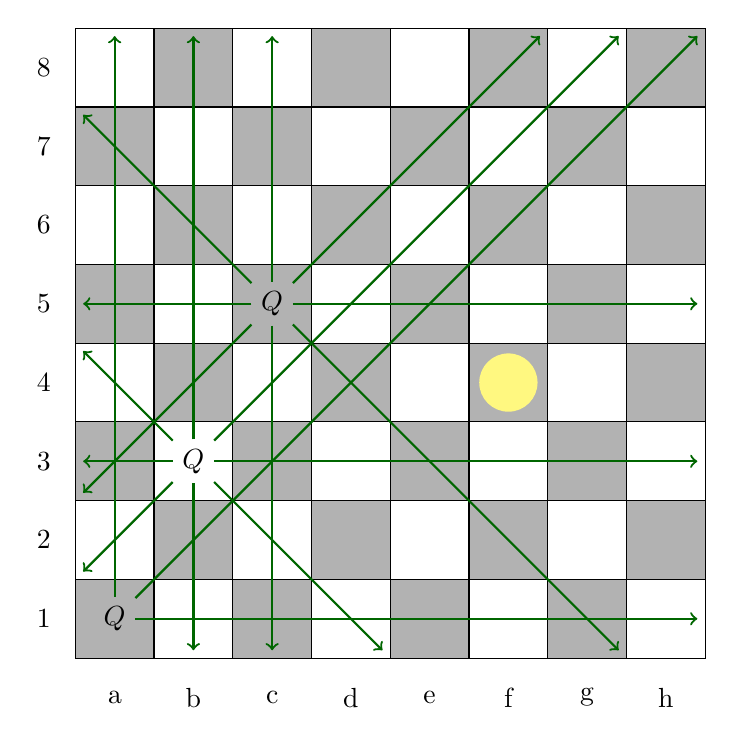
\begin{tikzpicture}[line/.style={color=black!60!green,->,thick},x=1cm,y=1cm]
		\draw[fill=black!30,even odd rule] (0,0)
		foreach \n in {1,2,3,4} { -- ++ (8,0) -- ++ (0,1) -- ++ (-8,0) -- ++ (0,1) } -- (8,8)

		foreach \in in {1,2,3,4} { -- ++ (0,-8) -- ++ (-1,0) -- ++ (0,8) -- ++ (-1,0) } -- cycle

		foreach[count=\n] \m in {a,b,...,h} { (-0.4,\n-0.5) node {\n} (\n-0.5,-0.5) node {\m} };
		\node (Q1) at (0.5,0.5) {$Q$};
		\node (Q2) at (1.5,2.5) {$Q$};
		\node (Q3) at (2.5,4.5) {$Q$};
		
		%Q1 lines
		\draw[line] (Q1) -- (7.9,0.5);
		\draw[line] (Q1) -- (0.5,7.9);
		\draw[line] (Q1) -- (7.9,7.9);
		
		%Q2 lines
		\draw[line] (Q2) -- (0.1,1.1);
		\draw[line] (Q2) -- (6.9,7.9);
		\draw[line] (Q2) -- (0.1,3.9);
		\draw[line] (Q2) -- (3.9,0.1);
		\draw[line] (Q2) -- (1.5,7.9);
		\draw[line] (Q2) -- (1.5,0.1);
		\draw[line] (Q2) -- (0.1,2.5);
		\draw[line] (Q2) -- (7.9,2.5);

		%Q3 lines
		\draw[line] (Q3) -- (0.1,2.1);
		\draw[line] (Q3) -- (0.1,6.9);
		\draw[line] (Q3) -- (5.9,7.9);
		\draw[line] (Q3) -- (6.9,0.1);
		\draw[line] (Q3) -- (0.1,4.5);
		\draw[line] (Q3) -- (2.5,0.1);
		\draw[line] (Q3) -- (2.5,7.9);
		\draw[line] (Q3) -- (7.9,4.5);
		
		\node[circle,fill=yellow!50] (') at (5.5,3.5) {$\ \ \ \ $};
		
	\end{tikzpicture}
\end{document}
